\chapter{Matematický model}
\label{kap:matematicky_model}
V tejto kapitole odvodíme rovnice obálky pre jednoparametrický systém elíps a elipsoidov. Najprv však klasifikujme krivky a plochy druhého stupňa. Nasledujúca teória a klasifikácia nadplôch druhého rádu je prevzatá zo \cite{Ivan}, \cite{Kor13}, \cite{Gla16}, \cite{Ode20} a \cite{Zla11}.
\section{Krivky druhého stupňa}
Krivka druhého stupňa $p$ je v karteziánskych súradniciach $(x, y) \in \mathbb{E}^2$ daná rovnicou 
$$ f(x, y) = Ax^2 + Bxy + Cy^2 + Dx + Ey + F = 0.$$
Prípad $A = B = C = 0$  môžeme vylúčiť, pretože potom je rovnica lineárna a opisuje priamku. Vo všeobecnosti rovnica vyjadruje kužeľosečku, ktorá je daná piatimi bodmi. Ak $F \neq 0$, môžeme ju vydeliť $F$ a potom riešiť sústavu lineárnych rovníc s piatimi neznámymi. Okrem klasických prípadov, ako elipsy, paraboly a hyperboly, môžu kužeľosečky degenerovať na dvojice priamok, bod alebo prázdnu množinu.

V algebraickom zmysle má kužeľosečka $p$ vždy dva priesečníky $S_1$ a $S_2$ s danou priamkou $s$. Oba môžu byť reálne alebo komplexne združené. Limitný prípad $S_1 = S_2$ nastáva vtedy, keď $s$ je dotyčnicou ku $p$.

V závislosti od počtu reálnych priesečníkov s priamkou $s$ v nekonečne rozlišujeme tri typy kužeľosečiek 
\begin{enumerate}
\item eliptický typ: bez reálnych priesečníkov,
\item hyperbolický typ: dva reálne priesečníky,
\item parabolický typ: priamka v nekonečne sa dotýka krivky.
\end{enumerate}

\begin{definition}
Matica $M \in \mathbb{R}^{n \times n}$ sa nazýva ortogonálna, ak platí $M^T M = I_n$, alebo, čo je to isté, $M^{-1} = M^T$. 
\end{definition}
Prvá podmienka hovorí, že stĺpce matice $M$ tvoria ortonormálnu bázu euklidovského priestoru $\mathbb{R}^n$ so štandardným skalárnym súčinom. Potom tiež platí $MM^T = I_n$, teda takisto riadky matice $M$ tvoria ortonormálnu bázu v $\mathbb{R}^n$. 

\begin{theorem} 
Matica prechodu od ortonormálnej bázy v $\mathbb{R}^n$ so štandardným skalárnym súčinom k ortonormálnej báze je ortogonálna matica. Tiež, ak od ortonormálnej bázy v $\mathbb{R}^n$ prejdeme pomocou ortogonálnej matice prechodu k novej báze,
tak aj nová báza bude ortonormálna.
\end{theorem}

\subsection{Invarianty kriviek druhého stupňa}
\begin{definition}
Invariantom krivky druhého stupňa $p$, vyjadrenej rovnicou
$$
f(x, y) = a_{11}x^2 + 2a_{12}xy + a_{22}y^2 + 2a_{13}x + 2a_{23}y + a_{33} = 0
$$
je každý taký algebraický výraz, závisiaci od \(a_{11}, a_{12}, a_{22}, a_{13}, a_{23}, a_{33}\), ktorého hodnota sa nezmení, ak túto krivku vyjadríme v inom karteziánskom súradnicovom systéme, ku ktorému prejdeme pomocou otočení alebo posunutí (čím od rovnice, viažúcej staré premenné \(x, y\), prejdeme k rovnici, viažúcej nové premenné \(x', y'\)).
\end{definition}

\begin{theorem}
Nasledujúce číselné výrazy sú invariantmi krivky druhého stupňa, vyjadrenej rovnicou $f(x, y)$.
\begin{align*}
\Delta &= \det \begin{pmatrix} 
a_{11} & a_{12} & a_{13} \\ 
a_{12} & a_{22} & a_{23} \\
a_{13} & a_{23} & a_{33} \end{pmatrix}, \
\delta = \det \begin{pmatrix} a_{11} & a_{12} \\ a_{12} & a_{22} \end{pmatrix}, \
s = a_{11} + a_{22}.
\end{align*}
\end{theorem}
Z tohto možno odvodiť nasledujúcu klasifikáciu kužeľosečiek.

%\begin{table}[h]
%\centering
%\begin{tabular}{|c|c|c|l|}
%\hline
%\textbf{Typ} & $\delta$ & $\Delta$ & \textbf{Tvar}  \\
%\hline
%\multirow{3}{*}{eliptický} & \multirow{3}{*}{$> 0$} & $\neq 0$ & ak $s\Delta < 0$, tak elipsa \\
%& & $\neq 0$ & ak $s\Delta > 0$, tak  $\emptyset$ \\
%& & $= 0$ & bod \\
%\hline
%\multirow{2}{*}{hyperbolický} & \multirow{2}{*}{$< 0$} & $\neq0$ & hyperbola \\
% & & $=0$ & dve rôznobežné priamky \\
%\hline
%\multirow{4}{*}{parabolický} & \multirow{4}{*}{$= 0$} & $\neq0$ & parabola \\
%& & $=0$ & dve rovnobežné priamky \\
%& & $= 0$ & priamka \\
%& & $= 0$ & $\emptyset$ \\
%\hline
%\end{tabular}
%\caption{Klasifikácia kužeľosečiek.}
%\label{tab:conic_sections}
%\end{table}

\begin{table}[h]
\centering
\begin{tabular}{|l|l|l|l|}
\hline
\textbf{Typ} & $\delta$ & $\Delta \neq  0$ & $\Delta = 0 $ \\
\hline
\multirow{2}{*}{eliptický} & \multirow{2}{*}{$> 0$} & ak $s\Delta < 0$, tak elipsa & \multirow{2}{*}{bod} \\
& & ak $s\Delta > 0$, tak $\emptyset$ & \\
\hline
hyperbolický & $< 0$ & hyperbola & dve rôznobežné priamky \\
\hline
\multirow{3}{*}{parabolický} & \multirow{3}{*}{$= 0$} & dve rovnobežné priamky & \multirow{3}{*}{parabola} \\
& & priamka & \\
& & $\emptyset$ & \\
\hline
\end{tabular}
\caption{Klasifikácia kužeľosečiek.}
\label{tab:conic_sections}
\end{table}

\section{Plochy druhého stupňa}
Plocha druhého stupňa $P$ je v karteziánskych súradniciach $(x, y, z) \in \mathbb{E}^3$ daná rovnicou
\[ f(x, y, z) = Ax^2 + By^2 + Cz^2 + Dxy + Exz + Fyz + Gx + Hy + Iz + J = 0. \]
Je zrejmé, že ak je prvých šesť koeficientov nulových, uvedená rovnica je lineárna a opisuje rovinu v priestore. Vo všeobecnosti rovnica opisuje kvadriku, ktorá je daná deviatimi bodmi. Ak $J \neq 0$, môžeme ju vydeliť $J$ a potom vyriešiť sústavu lineárnych rovníc s deviatimi neznámymi. Okrem klasických prípadov, ako elipsoidy, paraboloidy a hyperboloidy, môžu kvadriky degenerovať aj na kvadratické kužele, kvadratické valce a dvojice rovín.

V algebraickom zmysle je kvadrika $P$ plocha druhého stupňa, ktorá má vždy dva priesečníky $S-1$ a $S_2$ s danou priamkou $s$. Oba môžu byť reálne alebo komplexne združené. Limitný prípad $S_1 = S_2$ nastáva vtedy, keď $s$ je dotyčnicou $P$.

V závislosti od počtu reálnych priesečníkov s rovinou $s$ v nekonečne rozlišujeme tri typy kvadrík:
\begin{enumerate}
\item eliptický typ: bez reálnych priesečníkov,
\item hyperbolický typ: dva reálne priesečníky,
\item parabolický typ: kvadriky sa dotýka rovina v nekonečne.
\end{enumerate}
\subsection{Invarianty plôch druhého stupňa}
Nasledujúce číselné výrazy sú invariantmi plochy druhého stupňa $P$, vyjadrenej rovnicou 
\[ f(x, y, z) = a_{11}x^2 + a_{22}y^2 + a_{33}z^2 + 2a_{12}xy + 2a_{13}xz + 2a_{23}yz + 2a_{14}x + 2a_{24}y + 2a_{23}z + a_{44} = 0. \]
\begin{align*}
\Delta &= \det M = \det \begin{pmatrix} 
a_{11} & a_{12} & a_{13} & a_{14} \\ 
a_{21} & a_{22} & a_{23} & a_{24} \\
a_{31} & a_{32} & a_{33} & a_{34} \\
a_{41} & a_{42} & a_{43} & a_{44}
\end{pmatrix}, \
\delta = \det \begin{pmatrix} 
a_{11} & a_{12} & a_{13} \\ 
a_{21} & a_{22} & a_{23} \\ 
a_{31} & a_{32} & a_{33} 
\end{pmatrix}
\end{align*}
\begin{align*}
T &= \det \begin{pmatrix} 
a_{11} & a_{12} \\ 
a_{21} & a_{22} 
\end{pmatrix} + \det \begin{pmatrix} 
a_{22} & a_{23} \\ 
a_{32} & a_{33} 
\end{pmatrix} + \det \begin{pmatrix} 
a_{33} & a_{31} \\ 
a_{13} & a_{11} 
\end{pmatrix}, 
\end{align*}
\begin{align*}
s &= a_{11} + a_{22} + a_{33}, \ S = \Delta_{11} + \Delta_{22} + \Delta_{33}, 
\end{align*}
kde $ \Delta_{ij} $ je algebraický doplnok k prvku $a_{ij}$ matice $M, $ teda $\Delta_{ij} = (-1)^{i+j} \det(M_{ij}), $ kde $M_{ij}$ vznikne vyškrtnutím $i-$teho riadku a $j-$teho stĺpca.

Z tohto možno odvodiť nasledujúce dve tabuľky.

\begin{table}[H]
\centering
\begin{tabular}{|c|c|c|p{2.2cm}|p{2.15cm}|p{2cm}|}
\hline
Typ & $\delta$ & $s\delta$ a $T$ & $\Delta > 0$ & $\Delta < 0$ & $\Delta = 0$ \\
\hline
eliptický & $\neq 0$ & $s\delta>0$ a $T>0$ & $\emptyset$ & elipsoid & $\emptyset$ \\
\hline
hyperbolický & $\neq 0$ & $s\delta<0$ alebo $T \leq0$ & jednodielny hyperboloid & dvojdielny hyperboloid & kužeľ \\
\hline
parabolický & $=0$ & & hyperbolický paraboloid & eliptický paraboloid & valcové a reducibilné plochy \\
\hline
\end{tabular}
\caption{Klasifikácia kvadrík.}
\label{tab:classification_of_quadrics}
\end{table}

%\begin{table}[h]
%\begin{adjustbox}{center}
%\centering
%\begin{tabular}{|c|c|c|p{2.2cm}|p{2.15cm}|p{2cm}|}
%\hline
%Typ & $\delta$ & $s\delta$ a $T$ & $\Delta > 0$ & $\Delta < 0$ & $\Delta = 0$ \\
%\hline
%eliptický & $\neq 0$ & $s\delta>0$ a $T>0$ & $\emptyset$ & elipsoid & $\emptyset$ \\
%\hline
%hyperbolický & $\neq 0$ & $s\delta>0$ alebo $T \leq0$ & jednodielny hyperboloid & dvojdielny hyperboloid & kužeľ \\
%\hline
%parabolický & $=0$ & & hyperbolický paraboloid & eliptický paraboloid & valcové a reducibilné plochy \\
%\hline
%\end{tabular}
%\end{adjustbox}
%\caption{Klasifikácia kvadrík.}
%\label{tab:classification_of_quadrics}
%\end{table}

Pre valcové a reducibilné plochy máme ďalšie rozdelenie.

\begin{table}[H]
\centering
\begin{tabular}{|l|l|l|l|}
\hline
Typ & $T$ & $S \neq  0$ & $S = 0 $ \\
\hline
\multirow{2}{*}{eliptický} & \multirow{2}{*}{$> 0$} & ak $s\Delta < 0$, tak eliptický valec & \multirow{2}{*}{bod} \\
& & ak $s\Delta > 0$, tak $\emptyset$ &\\
\hline
hyperbolický & $< 0$ & hyperbolický valec & dve rôznobežné roviny \\
\hline
\multirow{3}{*}{parabolický} & \multirow{3}{*}{$= 0$} & \multirow{3}{*}{parabolický valec} & dve rovnobežné roviny \\
& & & rovina \\
& & & $\emptyset$ \\
\hline
\end{tabular}
\caption{Klasifikácia valcových a reducibilných plôch.}
\label{tab:degenerate_quadrics}
\end{table}

\section{Obálka elíps}
Pre vyriešenie úlohy zostrojenia obálky elipsoidov sme sa najprv zaoberali obálkou elíps.

Nech $M(t) \colon I \subset \mathbb{R} \rightarrow \mathbb{R}^{3 \times 3}$ je jednoparametrický systém (nie nutne regulárnych) symetrických $3 \times 3$ matíc. Nech $ X = (x, y, 1)^T$ sú homogénne súradnice v $\mathbb{P}^2(\mathbb{R})$, potom
\begin{equation*}
Q(t) \colon X^T M(t) X = 0 
\end{equation*}
je rovnica jednoparametrického systému kužeľosečiek. 
Matica $M(t)$ je tvaru
$$
\left(\begin{matrix} 
A(t) & \frac{B(t)}{2} & \frac{D(t)}{2} \\
\frac{B(t)}{2} & C(t) & \frac{E(t)}{2} \\
\frac{D(t)}{2} & \frac{E(t)}{2} & F(t) 
\end{matrix} \right),
$$
kde jej prvky $A(t), \dots, F(t)$ sú diferencovateľné funkcie parametra $t \in I,$ ktoré definujú elipsu $Q_t$ danú funkciou 
$$f(x, y, t) = A(t)x^2 + B(t)xy + C(t)y^2 + D(t)x + E(t)y + F(t) = 0.$$
Deriváciu jednoparametrického systému $Q(t)$ vzhľadom na parameter $t$ označíme
\begin{equation*}
\dot{Q}(t) \colon X^T \dot{M}(t) X = 0.
\end{equation*}
Matica $\dot{M}(t)$ je tvaru
$$
\left(\begin{matrix} 
\dot{A}(t) & \frac{\dot{B}(t)}{2} & \frac{\dot{D}(t)}{2} \\
\frac{\dot{B}(t)}{2} & \dot{C}(t) & \frac{\dot{E}(t)}{2} \\
\frac{\dot{D}(t)}{2} & \frac{\dot{E}(t)}{2} & \dot{F}(t) 
\end{matrix} \right),
$$
kde jej prvky $\dot{A}(t), \dots, \dot{F}(t)$ sú funkcie parametra $t \in I,$ ktoré definujú kužeľosečku $\dot{Q}_t$ danú rovnicou 
$$\dfrac{\partial f(x, y, t)}{\partial t} = \dot{A}(t)x^2 + \dot{B}(t)xy + \dot{C}(t)y^2 + \dot{D}(t)x + \dot{E}(t)y + \dot{F}(t) = 0.$$

Označme determinant matice 
$$\Delta(t) \vcentcolon = \det \dot{M}(t) $$
a subdeterminant matice, ktorá vznikne odstránením tretieho riadku a tretieho stĺpca 
$$\delta(t) \vcentcolon = \det \dot{M}_{33}(t).$$ 

\subsection{Zmena bázy elíps}
Nech $m(t) \colon  I \subseteq \mathbb{R} \rightarrow \mathbb{R}^2$ je aspoň dvakrát diferencovateľná krivka, napíšme rovnicu jednoparametrického systému elíps $Q$ so stredom na krivke $m(t)$, hlavnou polosou $a$ v smere vektora $\dot{m}(t)$ a vedľajšou polosou $b$ v smere normálového vektora $\vec{n}$ ku krivke $m(t)$. Uvažujme $\vec{n}=(-\dot{m}_2, \dot{m}_1). $ Vydelením normou vektorov $\dot{m}(t)$ a $\vec{n}$ dostávame novú ortonormálnu bázu tvorenú stĺpcovými vektormi matice $P(t),$ kde
$$
P(t) = \frac{1}{ \| \dot{m}(t) \|} \left(\begin{matrix}
   \dot{m}_1(t) & -\dot{m}_2(t) \\
   \dot{m}_2(t) & \dot{m}_1(t)
\end{matrix} \right).
$$
Keďže sme prešli od štandardnej bázy k ortonormálnej báze, matica $P(t)$ je ortogonálna, a teda
$$
P^{-1} = P^{T} = \frac{1}{ \| \dot{m}(t) \|} \left(\begin{matrix}
  \dot{m}_1(t) & \dot{m}_2(t) \\
  -\dot{m}_2(t) & \dot{m}_1(t)
\end{matrix}\right).
$$
V súradniciach $(u(t), v(t))$ má systém $Q$ rovnicu v kanonickom tvare 
\begin{align*}
\frac{u^2(t)}{a^2} + \frac{v^2(t)}{b^2} = 1,
\end{align*}
kde vzťah medzi súradnicami $(u(t), v(t))$ a $(x,y)$ je daný
$$
\left(\begin{matrix}
u(t) \\
v(t)
\end{matrix}\right) = \frac{1}{ \| \dot{m}(t) \|}
\left(\begin{matrix}
  \dot{m}_1(t) & \dot{m}_2(t) \\
   -\dot{m}_2(t) & \dot{m}_1(t)
\end{matrix}\right)
\left(\begin{matrix} \left(\begin{matrix} x \\ y \end{matrix}\right) - \left(\begin{matrix} m_1(t) \\ m_2(t) \end{matrix}\right) \end{matrix}\right).
$$
Systém elíps $Q$ sa potom transformuje na tvar
\begin{align} 
\label{eq:elipsa_v_novej_baze}
&\frac{1}{\|{\dot{m}}\|^2} \left( (x - m_1)^2 \left( \frac{{\dot{m}_1}^2}{a^2} + \frac{{\dot{m}_2}^2}{b^2} \right) + (y - m_2)^2 \left( \frac{{\dot{m}_2}^2}{a^2} + \frac{{\dot{m}_1}^2}{b^2} \right) \right) \notag \\
+ &\frac{1}{\|{\dot{m}}\|^2} \left( 2\left( \frac{1}{a^2} - \frac{1}{b^2} \right)(x - m_1)(y - m_2)\dot{m}_1\dot{m}_2 \right) - 1 = 0,
\end{align}
po miernej úprave tak dostávame výraz
\begin{align*} 
&\frac{1}{a^2b^2\|\dot{m}\|^2} \left( (x - m_1)^2 \left( b^2 \dot{m}_1^2 + a^2 \dot{m}_2^2 \right) + (y - m_2)^2 \left( a^2 \dot{m}_1^2 + b^2 \dot{m}_2^2 \right) \right) \\
+ &\frac{1}{a^2b^2\|\dot{m}\|^2} \left( 2(b^2 - a^2)(x - m_1)(y - m_2)\dot{m}_1\dot{m}_2 \right) - 1 = 0.
\end{align*}

\subsection{Výpočet obálky elíps}
Prepíšme jednoparametrický systém elíps $Q$ v novej báze, teda rovnicu \ref{eq:elipsa_v_novej_baze}, do maticového zápisu.
\begin{align*}
A &= \frac{b^2 \dot{m}_1^2 + a^2 \dot{m}_2^2}{a^2b^2 \| \dot{m} \|^2} \\
B &= \frac{2(b^2-a^2)\dot{m}_1 \dot{m}_2}{a^2b^2 \| \dot{m} \|^2} \\
C &= \frac{a^2 \dot{m}_1^2 + b^2 \dot{m}_2^2}{a^2b^2\| \dot{m} \|^2} \\
D &= \frac{- 2m_1 \left( b^2 \dot{m}_1^2 + a^2 \dot{m}_2^2 \right) - 2 \left(b^2 - a^2 \right) m_2 \dot{m}_1 \dot{m}_2 }{a^2b^2\| \dot{m} \|^2} \\
E &= \frac{- 2m_2 \left( a^2 \dot{m}_1^2 + b^2 \dot{m}_2^2 \right) - 2 \left(b^2 - a^2 \right) m_1 \dot{m}_1 \dot{m}_2 }{a^2b^2\| \dot{m} \|^2} \\
F &= \frac{\dot{m}_1^2 (b^2 m_1^2 + a^2 m_2^2 - a^2b^2) + 2 (b^2 - a^2) m_1 m_2 \dot{m}_1 \dot{m}_2 + \dot{m}_2^2 (a^2 m_1^2 + b^2 m_2^2 - a^2b^2) }{a^2b^2\| \dot{m}  \|^2}  -  1.  \\
\end{align*}
Derivujme funkcie $A(t), \dots, F(t).$ 
\begin{flalign*}
&\dot{A} = \frac{2 ( b^2 - a^{2}) ( \ddot{m}_{1} \dot{m}_{2} - \dot{m}_{1} \ddot{m}_{2}) \dot{m}_{1} \dot{m}_{2}}{a^{2} b^{2} \|\dot{m} \|^4} & \\
&\dfrac{\dot{B}}{2} = \frac{(a^{2} - b^{2}) (2 (\dot{m}_{1} \ddot{m}_{1} + \dot{m}_{2} \ddot{m}_{2}) \dot{m}_{1} \dot{m}_{2} - (\dot{m}_{1} \ddot{m}_{2} + \ddot{m}_{1} \dot{m}_{2}) \|\dot{m} \|^2)}{a^{2} b^{2} \|\dot{m} \|^4} & \\
&\dot{C} = \frac{2 (b^2 - a^{2}) ( \dot{m}_{1} \ddot{m}_{2} - \ddot{m}_{1} \dot{m}_{2}) \dot{m}_{1} \dot{m}_{2}}{a^{2} b^{2} \|\dot{m} \|^4} & \\
\end{flalign*}

\begin{flalign*}
& \dfrac{\dot{D}}{2} = \frac{2(\dot{m}_{1} \ddot{m}_{1} + \dot{m}_{2} \ddot{m}_{2}) (a^{2} (m_{1} \dot{m}_{2} - m_{2} \dot{m}_{1}) \dot{m}_{2} + b^{2} (m_{1} \dot{m}_{1} + m_{2} \dot{m}_{2}) \dot{m}_{1})}{a^{2} b^{2} \|\dot{m} \|^4} & \\
&- \frac{\|\dot{m} \|^2 (a^{2}(m_{1} \dot{m}_{2} - m_{2} \dot{m}_{1}) \ddot{m}_{2} + a^2 (m_{1} \ddot{m}_{2} - m_{2} \ddot{m}_{1}) \dot{m}_{2})}{a^{2} b^{2} \|\dot{m} \|^4} & \\
&- \frac{\|\dot{m} \|^2 ( b^{2}(m_{1} \dot{m}_{1} + m_{2} \dot{m}_{2}) \ddot{m}_{1} + b^2 (m_{1} \ddot{m}_{1} + m_{2} \ddot{m}_{2} + \|\dot{m} \|^2) \dot{m}_{1})}{a^{2} b^{2} \|\dot{m} \|^4} & \\
& \dfrac{\dot{E}}{2} = \frac{- 2 (\dot{m}_{1} \ddot{m}_{1} + \dot{m}_{2} \ddot{m}_{2}) (a^{2} (m_{1} \dot{m}_{2} - m_{2} \dot{m}_{1}) \dot{m}_{1} - b^{2} (m_{1} \dot{m}_{1} + m_{2} \dot{m}_{2}) \dot{m}_{2})}{a^{2} b^{2} \|\dot{m} \|^4} & \\
&+ \frac{\|\dot{m} \|^2 (a^{2} (m_{1} \dot{m}_{2} - m_{2} \dot{m}_{1}) \ddot{m}_{1} + a^{2} (m_{1} \ddot{m}_{2} - m_{2} \ddot{m}_{1}) \dot{m}_{1})}{a^{2} b^{2} \|\dot{m} \|^4} & \\
&- \frac{\|\dot{m} \|^2 (b^{2} (m_{1} \dot{m}_{1} + m_{2} \dot{m}_{2}) \ddot{m}_{2} + b^{2} (m_{1} \ddot{m}_{1} + m_{2} \ddot{m}_{2} + \|\dot{m} \|^2) \dot{m}_{2})}{a^{2} b^{2} \|\dot{m} \|^4} & \\
& \dot{F} = \frac{-2(\dot{m}_{1} \ddot{m}_{1} + \dot{m}_{2} \ddot{m}_{2}) (- a^{2} b^{2} \|\dot{m} \|^2 + a^{2} (m_{1}\dot{m}_{2} - m_{2}\dot{m}_{1})^2 + b^{2} (m_{1} \dot{m}_{1} + m_{2} \dot{m}_{2})^{2})}{a^{2} b^{2} \|\dot{m} \|^4} & \\
&+ \frac{ \|\dot{m} \|^2 (- a^{2} b^{2} (\dot{m}_{1} \ddot{m}_{1} + \dot{m}_{2} \ddot{m}_{2}) + a^{2} (m_{1}^{2} \dot{m}_{2} \ddot{m}_{2} - m_{1} m_{2} \dot{m}_{1} \ddot{m}_{2} - m_{1} m_{2} \ddot{m}_{1} \dot{m}_{2} + m_{2}^{2} \dot{m}_{1} \ddot{m}_{1})}{a^{2} b^{2} \|\dot{m} \|^4} & \\
&+ \frac{ \|\dot{m} \|^2 b^{2} (m_{1}^{2} \dot{m}_{1} \ddot{m}_{1} + m_{1} m_{2} \dot{m}_{1} \ddot{m}_{2} + m_{1} m_{2} \ddot{m}_{1} \dot{m}_{2} + m_{1}\dot{m}_{1}^{3})}{a^{2} b^{2} \|\dot{m} \|^4} & \\
&+ \frac {\|\dot{m} \|^2 b^{2} (m_{1} \dot{m}_{1} \dot{m}_{2}^{2} + m_{2}^{2} \dot{m}_{2} \ddot{m}_{2} + m_{2} \dot{m}_{1}^{2} \dot{m}_{2} + m_{2} \dot{m}_{2}^{3})}{a^{2} b^{2} \|\dot{m} \|^4}.
\end{flalign*}


Určme typ kužeľosečiek jednoparametrického systému $\dot{Q}$ podľa jeho invariantov.
Invarianty
\begin{flalign*}
&\Delta(t) = 0 & \\
&\delta(t) = \dot{A} \dot{C} - \frac{\dot{B}^2}{4} =  -\frac{(b^2 - a^2)^2}{a^4b^4} \frac{ (\dot{m_1}\ddot{m_2} - \ddot{m_1}\dot{m_2})^2 + \dot{m_1}\dot{m_2}\ddot{m_1}\ddot{m_2}}{\|m\|^4} < 0
\end{flalign*}
pre všetky $t,$ teda kužeľosečky v systéme $\dot{Q}$ podľa klasifikácie \ref{tab:conic_sections} degenerujú na dve rôznobežné priamky. 

%Ukázali sme, že jednoparametrický systém $\dot{Q}$ sú pre každý parameter dve rôznobežné priamky.

TO DO prienik $Q$ a $\dot{Q}$ a interpretácia výsledkov
\begin{example}[Parabola]
Majme parabolu s parametrizáciou $m(t)=(t, t^2), $ kde $\dot{m}(t)=(1, 2t).$ Transformujme jednoparametrický systém elíps $Q$.
\begin{align*}
Q: \quad &\frac{1}{a^{2} b^{2}\left(4 t^{2} + 1\right)} \left( (x-t)^2 (b^2 + a^{2} 4t^2) + (y-t^2)^2 (a^2 + b^2 4t^2) \right)\\
+ &\frac{1}{a^{2} b^{2}\left(4 t^{2} + 1\right)} \left( 4t(b^2 - a^2)(x-t)(y-t^2)2t \right) - 1 = 0.
\end{align*}
TO DO dokončiť príklad
\end{example}

%\begin{example}[Parabola]
%$$
%\frac{2 \cdot \left(2 a^{2} \cdot \left(2 t \left(t^{2} + 2 t \left(- t + x\right) - y\right) + \left(t - x\right) \left(4 t^{2} + 1\right)\right) \left(- t^{2} + 2 t \left(t - x\right) + y\right) + b^{2} \cdot \left(4 t \left(2 t \left(- t^{2} + y\right) - t + x\right) + \left(4 t^{2} + 1\right) \left(6 t^{2} - 2 y + 1\right)\right) \left(2 t \left(t^{2} - y\right) + t - x\right)\right)}{a^{2} b^{2} \left(4 t^{2} + 1\right)^{2}} = 0
%$$
%\end{example}

\section{Obálka elipsoidov}
Pododobne ako pre elipsy odvodíme formu zápisov s dorbnými úpravami pre elipsoidy. Pre tento prípad parameter $t$ pre lepšiu prehľadnosť vynechávame.
Nech $M(t) \colon I \subset \mathbb{R} \rightarrow \mathbb{R}^{4 \times 4}$ je jednoparametrický systém (nie nutne regulárnych) symetrických $4 \times 4$ matíc. Nech $ X = (x, y, z, 1)^T$ sú homogénne súradnice v $\mathbb{P}^3(\mathbb{R})$, potom
\begin{equation*}
Q(t) \colon X^T M(t) X = 0
\end{equation*}
je rovnica jednoparametrického systému elipsoidov. Matica $M(t)$ je tvaru
$$
\left(\begin{matrix} 
A & \frac{D}{2} & \frac{E}{2} & \frac{G}{2} \\
\frac{D}{2} & B & \frac{F}{2} & \frac{H}{2} \\
\frac{E}{2} & \frac{F}{2} & C & \frac{I}{2} \\
\frac{G}{2} & \frac{H}{2} & \frac{I}{2} & J \\
\end{matrix} \right),
$$
kde jej prvky $A, \dots, J$ sú diferencovateľné funkcie $A(t), \dots, J(t)$ parametra $t \in I,$ ktoré definujú elipsoid $Q_t$ daný funkciou 
$$
f(x, y, z, t) = Ax^2 + By^2 + Cz^2 + Dxy + Exz + Fyz + Gx + Hy + Iz + J = 0.
$$
Derivácia jednoparametrického systému $Q(t)$ vzhľadom na parameter $t$ je 
\begin{equation*}
\dot{Q}(t) \colon X^T \dot{M}(t) X = 0.
\end{equation*}
Matica $\dot{M}(t)$ je tvaru
$$
\left(\begin{matrix} 
\dot{A} & \frac{\dot{D}}{2} & \frac{\dot{E}}{2} & \frac{\dot{G}}{2} \\
\frac{\dot{D}}{2} & \dot{B} & \frac{\dot{F}}{2} & \frac{\dot{H}}{2} \\
\frac{\dot{E}}{2} & \frac{\dot{F}}{2} & \dot{C} & \frac{\dot{I}}{2} \\
\frac{\dot{G}}{2} & \frac{\dot{H}}{2} & \frac{\dot{I}}{2} & \dot{J} \\
\end{matrix} \right),
$$
kde jej prvky $A, \dots, F$ sú funkcie $\dot{A}(t), \dots, \dot{J}(t)$ parametra $t \in I,$ a definujú plochu druhého stupňa $Q_t$ danú rovnicou 
$$\dfrac{\partial f(x, y, z, t)}{\partial t} = \dot{A}x^2 + \dot{B}y^2 + \dot{C}z^2 + \dot{D}xy + \dot{E}xz + \dot{F}yz + \dot{G}x + \dot{H}y + \dot{I}z + \dot{J} = 0.$$
Označme determinant matice 
$$\Delta(t) \vcentcolon =  \det \dot{M}(t), $$
subdeterminant matice, ktorá vznikne odstránením štvrtého riadku a štvrtého stĺpca 
$$ \delta(t) \vcentcolon = \det \dot{M}_{44}(t) $$
%$$\delta(t) := \det \dot{M}_{44}(t),$$
%$$ T(t) = \left( \begin{bmatrix}
%\dot{A} & \dfrac{D}{2} \\ 
%\dot{\dfrac{D}{2}} & \dot{B}
%\end{bmatrix} right) + \left( \begin{bmatrix}
%\dot{B} & \dfrac{F}{2} \\ 
%\dot{\dfrac{F}{2}} & \dot{C}
%\end{bmatrix} right) + \left( \begin{bmatrix}
%\dot{C} & \dfrac{E}{2} \\ 
%\dot{\dfrac{E}{2}} & \dot{A}
%\end{bmatrix} right),$$
%$$ s(t) = A + B + C,
%$$ 
%$$
%\Delta'= \det \dot{M}_{11}(t) + \det \dot{M}_{22}(t) +\det \dot{M}_{33}(t).
%$$
a ďalšie invarianty plôch druhého stupňa
\begin{align*}
T(t) & = \det \left( \begin{matrix}
\dot{A} & \frac{\dot{D}}{2} \\ 
\frac{\dot{D}}{2} & \dot{B}
\end{matrix} \right) + \det \left( \begin{matrix}
\dot{B} & \frac{\dot{F}}{2} \\ 
\frac{\dot{F}}{2} & \dot{C}
\end{matrix} \right) + \det \left(  \begin{matrix}
\dot{C} & \frac{\dot{E}}{2} \\ 
\frac{\dot{E}}{2} & \dot{A}
\end{matrix} \right), \\
S(t) &= \det \dot{M}_{11}(t) + \det \dot{M}_{22}(t) + \det \dot{M}_{33}(t).
\end{align*}

\subsection{Zmena bázy elipsodiov}
Upravme rovnice pre obálku sféry tak, aby zodpovedali obálke elipsoidov. Vezmime sféru, zmeňme súradnicový systém so štandardnou bázou  $\vec{e}_1, \vec{e}_2, \vec{e}_3$ na lokálny súradnicový system krivky s bázou Frenetovho repéra $\vec{t}, \vec{n}, \vec{b}$ v každom bode krivky $m(t).$ Tak budeme môcť upraviť sféru na elipsoid tak, aby $a$ zodpovedalo škálovaniu v dotykovom smere priestorovej krivky $m(t)$ a $b$ zodpovedalo škálovaniu v normálovom a binormálovom smere. Frenetov repér je ortonormálna báza, ktorú tvoria stĺpcové vektory matice $P(t),$ kde
$$
P(t) = \left( \begin{matrix} \vec{t} & \vec{n} & \vec{b} \end{matrix} \right),
$$
kde
\begin{align*}
\vec{t} &= \dfrac{\dot{m}}{\| \dot{m} \|}, \\
\vec{n} &= \dfrac{\ddot{m} - \langle \ddot{m}, \vec{t} \rangle \vec{t}}{\| \ddot{m} - \langle \ddot{m}, \vec{t} \rangle \vec{t}\| }, \\
\vec{b} &= \dfrac{\dddot{m} - \langle \dddot{m}, \vec{t} \rangle \vec{t} - \langle \dddot{m}, \vec{n} \rangle \vec{n}}{\| \dddot{m} - \langle \dddot{m}, \vec{t} \rangle \vec{t} - \langle \dddot{m}, \vec{n} \rangle \vec{n} \| }.
\end{align*}
Matica $P(t)$ je ortogonálna, preto $P^{-1} = P^T.$
Keďže vyjadrenia nových vektorov sú pri prepise do súraníc alebo aj vyčíslení pre konkrétne prípady príliš dlhé, uvažujme inú ortonormálnu bázu, ktorá by zachovala požadované vlastnosti škálovania. Keďže je elipsoid v normálovom smere krivky homogénny, môžeme za $\vec{n}$ zvoliť ľubovoľný jednotkový vektor z normálovej roviny krivky. Vektor $\vec{b}$ následne zvolíme ako vektorový súčin $\vec{t} \times \vec{n}$ a normalizujeme ho. Uvažujme teda
\begin{align*}
\vec{t} &= \dfrac{(\dot{m}_1, \dot{m}_2, \dot{m}_3)}{\sqrt{\dot{m}_1^2 + \dot{m}_2^2 + \dot{m}_3^2}}, \\
\vec{n} &= \dfrac{(0, -\dot{m}_3, \dot{m}_2)}{\sqrt{\dot{m}_2^2 + \dot{m}_3^2}}, \\
\vec{b} &= \dfrac{(\dot{m}_2^2 + \dot{m}_3^2, -\dot{m}_1 \dot{m}_2, -\dot{m}_1 \dot{m}_3)}{\sqrt{\dot{m}_1^2 + \dot{m}_3^2}\sqrt{\dot{m}_1^2 + \dot{m}_2^2 + \dot{m}_3^2}},
\end{align*}
kde je $\dot{m_2} \neq 0$ a $\dot{m_3} \neq 0$. Ak by boli, vieme nájsť iné ortonormálne vektory $\vec{n}, \vec{b}$ v normálovej rovine krivky $m(t)$ podobného tvaru. 


Potom matica prechodu $P^{-1}$ má tvar
$$
P^{-1} = \left( \begin{matrix} \dfrac{\dot{m}_1}{\|\dot{m}\|} & \dfrac{\dot{m}_2}{\|\dot{m}\|} & \dfrac{\dot{m}_3}{\|\dot{m}\|} \\
0 & \dfrac{-\dot{m}_3}{\sqrt{\dot{m}_2^2 + \dot{m}_3^2}} & \dfrac{\dot{m}_2}{\sqrt{\dot{m}_2^2 + \dot{m}_3^2}} \\
\dfrac{\dot{m}_2^2 + \dot{m}_3^2}{\|\dot{m}\| \sqrt{\dot{m}_2^2 + \dot{m}_3^2}} & \dfrac{-\dot{m}_1 \dot{m}_2 }{\|\dot{m}\| \sqrt{\dot{m}_2^2 + \dot{m}_3^2}} &  \dfrac{-\dot{m}_1 \dot{m}_2}{ \|\dot{m}\| \sqrt{\dot{m}_2^2 + \dot{m}_3^2}} 
\end{matrix} \right).
$$
V súradniciach $(u(t),v(t),w(t))$ má jednoparametrický systém elipsoidov $Q$ rovnicu
\begin{align*}
\dfrac{u^2(t)}{a^2} + \dfrac{v^2(t)}{b^2} + \dfrac{w^2(t)}{b^2} = 1,
\end{align*}
kde vzťah medzi súradnicami $(u(t),v(t),w(t))$ a $(x,y,z)$ je daný
$$
\left(\begin{matrix}
u \\
v \\
w
\end{matrix}\right) = \frac{1}{ \| \dot{m}\| \sqrt{\dot{m}_2^2 + \dot{m}_3^2}}
\left( \begin{matrix} 
\dot{m}_1 \sqrt{\dot{m}_2^2 + \dot{m}_3^2} & \dot{m}_2 \sqrt{\dot{m}_2^2 + \dot{m}_3^2} & \dot{m}_3 \sqrt{\dot{m}_2^2 + \dot{m}_3^2} \\
0 & -\dot{m}_3 \| \dot{m}\| & \dot{m}_2 \| \dot{m}\| \\
\dot{m}_2^2 + \dot{m}_3^2 & -\dot{m}_1 \dot{m}_2 & -\dot{m}_1 \dot{m}_2 
\end{matrix} \right)
\left(\begin{matrix} x - m_1 \\ y - m_2 \\ z - m_3 \end{matrix}\right),
$$
Pre jednoparametrický systém elipsoidov $Q$ tak dostávame vyjadrenie
\begin{align*}
&\frac{- a^{2} b^{2} (\dot{m}_{2}^{2} + \dot{m}_{3}^{2}) \| \dot{m} \|^2 + a^{2} ((y - m_{2}) \dot{m}_{3} - (z - m_{3}) \dot{m}_{2})^{2} \| \dot{m} \|^2}{a^{2} b^{2} (\dot{m}_{2}^{2} + \dot{m}_{3}^{2}) \| \dot{m} \|^2} \\
+ &\frac{a^{2} (- (x - m_{1}) (\dot{m}_{2}^{2} + \dot{m}_{3}^{2}) + (y - m_{2}) \dot{m}_{1} \dot{m}_{2} + (z - m_{3}) \dot{m}_{1} \dot{m}_{3})^{2}}{a^{2} b^{2} (\dot{m}_{2}^{2} + \dot{m}_{3}^{2}) \| \dot{m} \|^2} \\
+ &\frac{b^{2} \| \dot{m} \|^2  ((x - m_{1}) \dot{m}_{1} + (y - m_{2}) \dot{m}_{2} + (z - m_{3}) \dot{m}_{3})^{2}}{a^{2} b^{2} (\dot{m}_{2}^{2} + \dot{m}_{3}^{2}) \| \dot{m} \|^2} = 0.
\end{align*}

\subsection{Výpočet obálky elipsodiov}
\begin{flalign*}
&A = \frac{b^{2} \dot{m}_1^{2} + a^{2} \dot{m}_2^{2} + a^{2} \dot{m}_3^{2}}{a^2 b^2 \| \dot{m} \|^2} & \\
&B = \frac{a^{2} \dot{m}_1^{2} + b^{2} \dot{m}_2^{2} + a^{2} \dot{m}_3^{2}}{a^2 b^2 \| \dot{m} \|^2} & \\
&C = \frac{a^{2} \dot{m}_1^{2} + a^{2} \dot{m}_2^{2} + b^{2} \dot{m}_3^{2}}{a^2 b^2 \| \dot{m} \|^2} & \\
& \frac{D}{2} = \frac{\left(b^2 - a^2\right)\dot{m}_1\dot{m}_2}{a^2b^2 \| \dot{m} \|^2} & \\
& \frac{E}{2} = \frac{\left(b^2 - a^2\right)\dot{m}_1\dot{m}_3}{a^2b^2 \| \dot{m} \|^2} & \\
& \frac{F}{2} = \frac{\left(b^2 - a^2\right)\dot{m}_2\dot{m}_3}{a^2b^2 \| \dot{m} \|^2} & \\
& \frac{G}{2} = - \frac{ a^2 m_1 \dot{m}_3^2 + (b^2 - a^2) m_3 \dot{m}_1 \dot{m}_3 +  a^2 m_1 \dot{m}_2^2 + ( b^2 - a^2) m_2 \dot{m}_1 \dot{m}_2 + b^2 m_1 \dot{m}_1^2}{a^2b^2 \| \dot{m} \|^2} & \\
& \frac{H}{2} = - \frac{a^2 m_2 \dot{m}_3^2 + (b^2 - a^2) m_3 \dot{m}_2 \dot{m}_3 + b^2 m_2 \dot{m}_2^2 + (b^2 - a^2) m_1 \dot{m}_1 \dot{m}_2 + a^2 m_2 \dot{m}_1^2}{ a^2 b^2 \| \dot{m} \|^2 } & \\
& \frac{I}{2} = - \frac {(b^2 m_3 \dot{m}_3^2 + (b^2 - a^2) m_2 \dot{m}_2 + (b^2 - a^2) m_1 \dot{m}_1) \dot{m}_3 + a^2 m_3 \dot{m}_2^2 + a^2 m_3 \dot{m}_1^2}{a^2 b^2 \| \dot{m} \|^2 } & \\
& J = \frac{(a^2 m_1^2 + a^2 m_2^2 + b^2 m_3^2 - a^2 b^2) \dot{m}_3^2 + 2 (b^2 -a^2) (m_2 m_3 \dot{m}_2 + m_1 m_3 \dot{m}_1) \dot{m}_3 } {a^2 b^2 \|\dot{m} \|^2} & \\
&+ \frac{(a^2 m_1^2 + b^2 m_2^2 + a^2 m_3^2 - a^2 b^2) \dot{m}_2^2 + 2 (b^2 - a^2) m_1 m_2 \dot{m}_1 \dot{m}_2 + (b^2 m_1^2 + a^2 m_2^2 + a^2 m_3^2 - a^2 b^2) \dot{m}_1^2}{a^2 b^2 \|\dot{m} \|^2}
\end{flalign*}

Ako v prípade elíps, derivujme funkcie $A(t), \dots, J(t).$

Poznámka: Vzťahy derivácii sú dosť dlhé. 

Určme typ kvadrík jednoparametrického systému $\dot{Q}$ podľa jeho invariantov.
Invarianty
\begin{align*}
\Delta (t) &= 0, \\
\delta (t)&=0, \\
T(t) & =  \dot{A} \dot{B} - \frac{\dot{D}^2}{4} + 
\dot{B} \dot{C} - \frac{\dot{F}^2}{4} + 
\dot{A} \dot{C} - \frac{\dot{E}^2}{4} < 0 \\
S(t) & < 0,
\end{align*}
pre všetky $t \in I,$
teda podľa klasifikácie plôch druhého stupňa \ref{tab:classification_of_quadrics} a \ref{tab:degenerate_quadrics} sú kvadriky v systéme $\dot{Q}$ dve rôznobežné roviny.

TO DO prienik $Q$ a $\dot{Q}$ a interpretácia výsledkov

\section{Softvér Maxima}
Na všetky výpočty v tejto kapitole bol použitý voľne dostupný softvér počítačovej algebry Maxima s grafickým užívateľským rozhraním wmMaxima. Celý balík a dokumentácia sú dostupné na \cite{MaximaDoc}, \cite{MaximaDownload}. Rovnice z Maximy boli prevedené do \LaTeX u pomocou Python skriptu \verb|conversion-to-latex.ipynb|, ktorý sa nachádza v GitHub repozitári \url{https://github.com/tutka13/Masters-Thesis/tree/main/symbolic-computations}.

\begin{figure}[h]
	\centering
	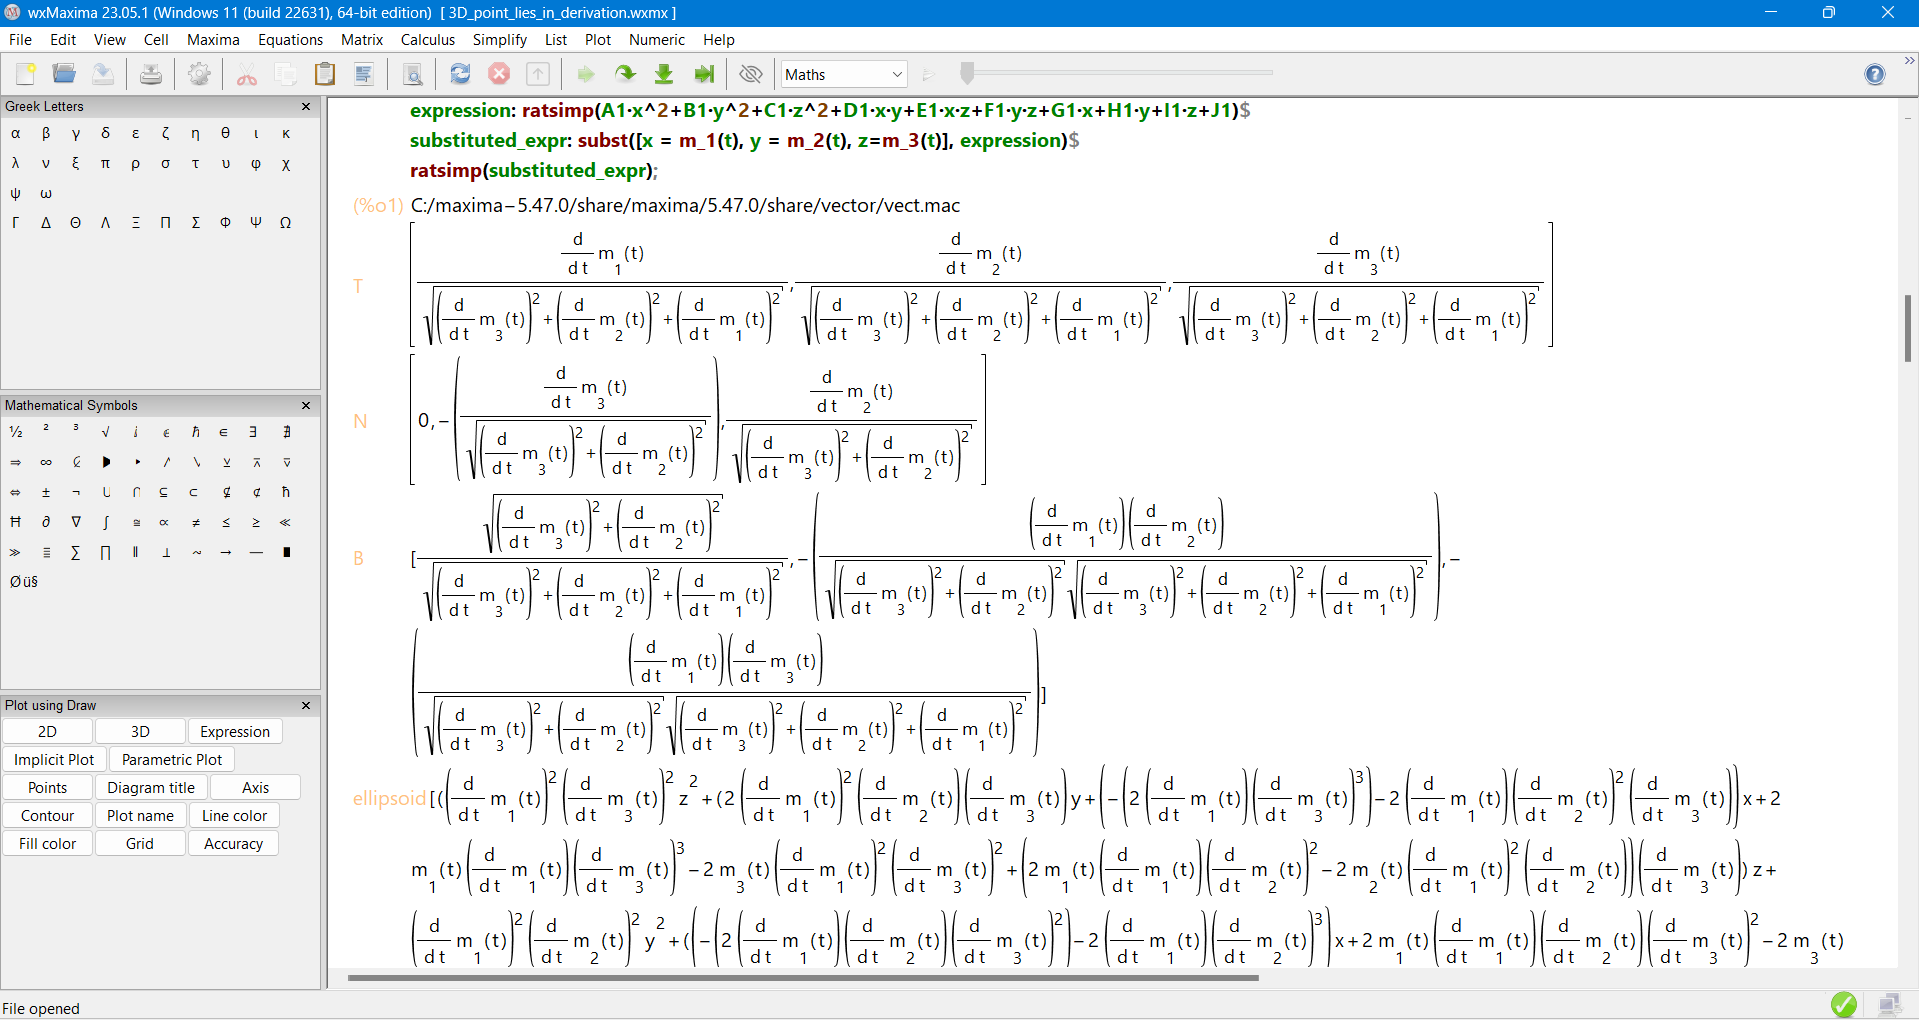
\includegraphics[width=\textwidth]{images/maxima.png}
	\caption[Softvér Maxima.]{Výpočet v softvéri Maxima.}
	\label{fig:3D_point_lies}
\end{figure}

